%! TEX root = main.tex

%/========== Introduction ==========/%

\chapter{Introduction}
% TODO: Introduce the thesis with a short, sweet, intuitive approach.
% No math, just whet the reader's appetite for what we are doing. What are the motivating examples? Why do we study what we study? Why choose VNHCs over other methods?
Consider a child who is standing on a swing.
Naturally, the child pushes off the ground and starts bending and extending
their knees; they swing higher and faster over time, until they 
have reached their express goal of going as high and fast as possible.

Now imagine that the child is a robot, and their creator is teaching them to
swing like a real boy.
The first thing the roboticist might do is plot the leg motion of a human child
as a function of time and have the robot synchronize with this plot.
In an ideal world, this technique would work perfectly and the robot boy would
swing high, experiencing the same soaring feeling as his human counterpart.

Unfortunately, this behaviour is entirely unnatural. 
Humans on swings do not bend or extend their knees at specific times; rather,
they adjust their leg position based on the current angle of the swing along
with their direction of motion, as in Figure \ref{fig:swing-pos-vel}.
This position-velocity adjustment allows humans to correct for external
disturbances (like strong winds or overly enthusiastic parents).
Even if the robot could perfectly track a time-based trajectory, an external
disturbance may desynchronize the leg motion with the swing to the point that
the swing will slow down rather than speed up.

\begin{figure}
    \centering
    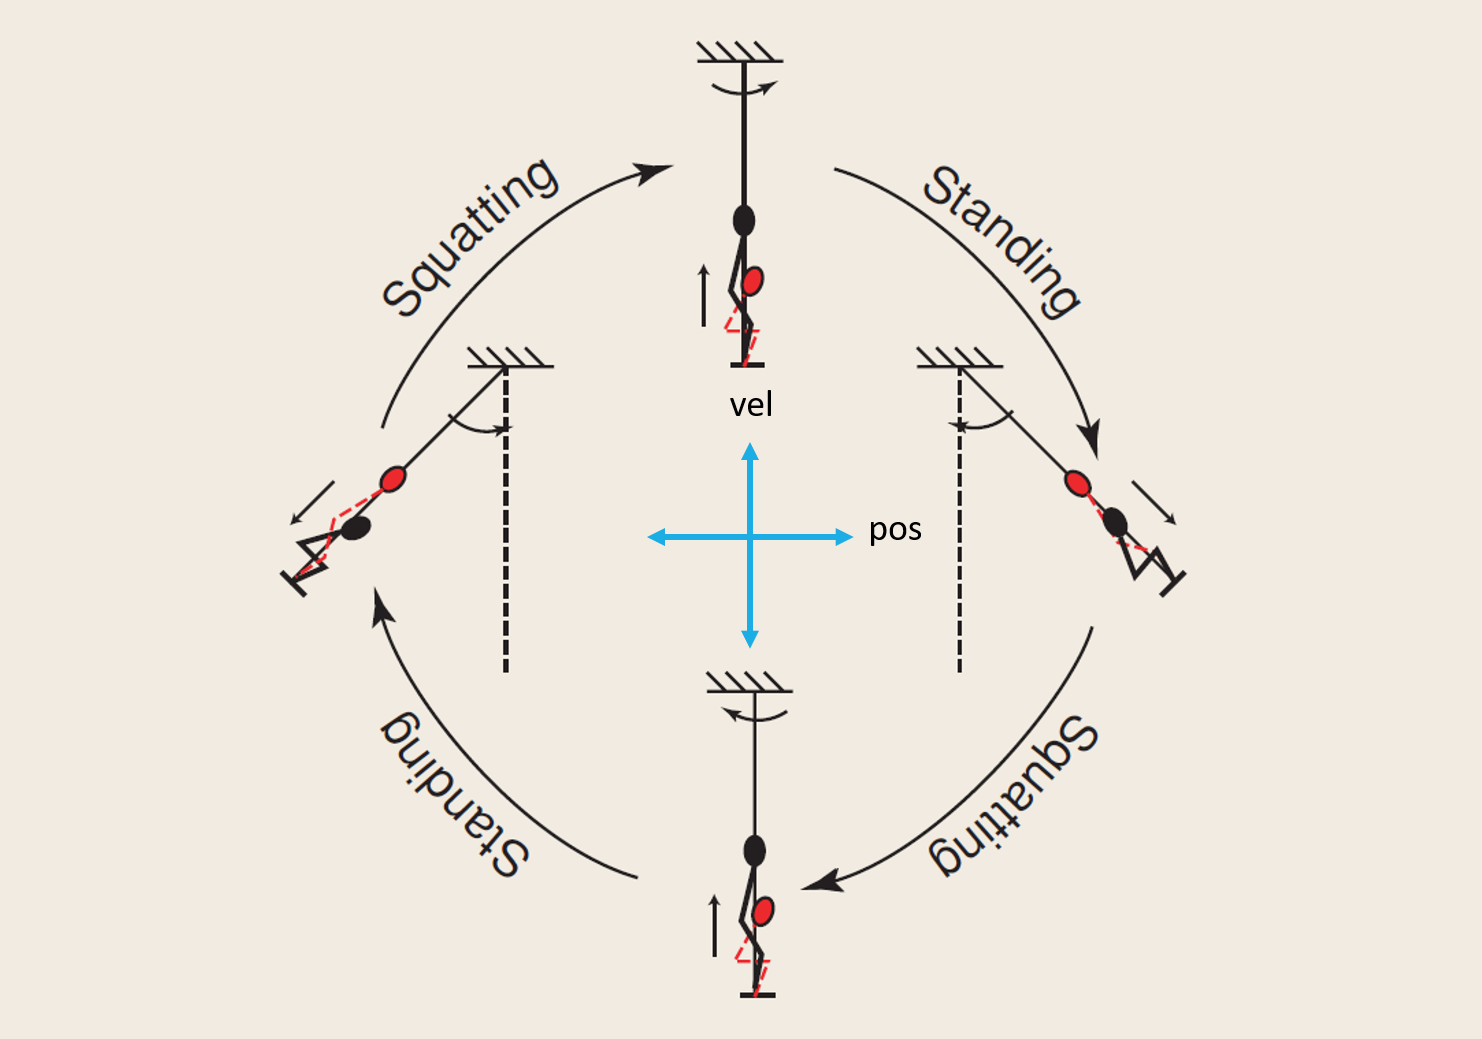
\includegraphics[width=0.75\textwidth]{images/swing_pos_vel.png}
    \caption{A person on a standing swing will squat as they approach the
        bottom of the swing path, and stand after they pass it until they hit
        the peak of their swing. Image taken (with modifications) from
    \cite{pumping_swing_standing_squatting}.}
    \label{fig:swing-pos-vel}
\end{figure}

One recent control technique known as \textit{virtual holonomic constraints}
forces a robot's actuators to track a function of position rather than time.
Sadly, this still won't do for our robot boy because a real child also bends
their knees according to their direction of motion.
In other words, the robot's legs need to move as a function not only of
position, but also of velocity.

These are the types of controllers we study in this thesis: they are called
\textit{virtual nonholonomic constraints}.

\section{Literature Review}

% TODO: write a brief lit review on energy injection and VNHCs.

\section{Statement of Contributions}
Here are the contributions of this thesis.
\begin{itemize}[label={}]
   \item \textbf{Chapter \ref{ch:vnhcs}} The development of the framework of
      virtual nonholonomic constraints.
      This includes the definition of simply actuated mechanical systems, virtual
      nonholonomic constraints, regular constraints, and energy injection.
      Theorem \ref{thm:vnhc-regularity} yields a characterization of regularity, 
      while Theorem \ref{thm:zero-dynamics} provides the constrained dynamics
      for a certain class of systems.
   \item \textbf{Chapter \ref{ch:vlp}} An application of virtual nonholonomic
      constraints to the variable-length pendulum, based on a pumping technique
      used by children on standing swings.
      The chapter culminates in Theorem \ref{thm:vlp-energy-stabilization},
      which guarantees that a certain class of VNHCs will inject energy into
      this system.
   \item \textbf{Chapter \ref{ch:acrobot}} An application of virtual
      nonholonomic constraints to the acrobot, where we develop a constraint
      by examining the intuitive motion performed by human gymnasts.
      The chapter ends with Theorem \ref{thm:acrobot-energy-stabilization},
      which proves that the constraint injects energy into the acrobot.
\end{itemize}

\section{Organization of the Thesis}
The thesis is laid out as such: 
in Chapter \ref{ch:vnhcs} we cover the requisite background on Hamiltonian
mechanics, after which we develop the main theory of virtual nonholonomic
constraints;
in Chapter \ref{ch:vlp} we reformulate a time-optimal energy-injection strategy
for the variable-length pendulum as a virtual nonholonomic constraint, and
prove that the pendulum will gain enough energy to rotate around the bar with
arbitrary speed;
and in Chapter \ref{ch:acrobot} we find a virtual nonholonomic constraint 
which enables the acrobot to kick its legs like a gymnast until it is
performing backflips on a horizontal bar.
Finally, we show experimental results for the acrobot which confirm that the
theory works in the real world.

%/========== /Introduction ==========/%
% vim: set tw=80 ts=4 sw=4 sts=0 et ffs=unix :
